\documentclass{beamer}
\usepackage[polish]{babel}
\usepackage[utf8]{inputenc}
\usepackage[T1]{fontenc}
\usepackage{svg}
\usepackage{animate}
\usepackage{graphicx}
\usetheme{Madrid}
\usecolortheme{default}
%------------------------------------------------------------
%This block of code defines the information to appear in the
%Title page
\title[Praca dyplomowa magisterska] %optional
{Analiza wykorzystania oscylatorów pierścieniowych jako źródła losowości w układach FPGA}
\subtitle{}
\author[Sz. Gogulski] % (optional)
{Szymon~Gogulski
\newline
\newline
Promotor: dr inż. Michał Melosik
\newline
\newline
Informatyka - Przetwarzanie Brzegowe
}
\institute[PP] % (optional)
{Politechnika Poznańska}
\date[Poznań 2026] % (optional)
{Praca dyplomowa Magisterska
\newline
Poznań 2026}
\logo{
\includegraphics[height=0.6cm]{pp_logo.pdf}}
\begin{document}
\frame{\titlepage}
%---------------------------------------------------------
\begin{frame}
\frametitle{Agenda}
\tableofcontents
\end{frame}
%---------------------------------------------------------
\section{Cel pracy}
%---------------------------------------------------------
\begin{frame}
\frametitle{Cel pracy}

\Large
\begin{itemize}
    \item Zbadać jak ilość oscylatorów pierścieniowych wpływa na jakość źródła entropii
    \item Opracować mechanizmy zawarte w SP 800-90B dla implementowanego źródła entropii (Health Test)
\end{itemize}

\end{frame}
%---------------------------------------------------------
\begin{frame}
\frametitle{Zadania Podstawowe}

\Large
\begin{itemize}
    \item Przygotować implementację układu w oparciu o płytę deweloperską,
    \item Przygotować środowisko testów urządzenia i zbierania danych,
    \item Opracować testy zdrowia dla modułu,
    \item Przeprowadzić badania.
\end{itemize}



\end{frame}
%---------------------------------------------------------
\begin{frame}
\frametitle{Zadania Ewentualne}

\Large

\begin{itemize}
    \item Zbadać wpływ metod postprocessingu na jakość źródła entropii,
    \item Przygotować implementacją do celów użytkowych, np. integracja z RPI,
    \item Porównanie wydajności z innym źródłem entropii.
\end{itemize}

\end{frame}
%---------------------------------------------------------
\section{Drugie seminarium}
%---------------------------------------------------------
\begin{frame}
\frametitle{NIST SP 800-90 A/B/C}
\Large
\begin{itemize}
    \item NIST - National Institute of Standards and Technology
    \item SP - special publication
    \item 800 - seria
    \item 90 - numer publikacji w serii
    \item A/B/C - część publikacji
\end{itemize}

\vspace{0.5cm}

NIST SP 800-90 - zbiór publikacji dotyczących generowania liczb losowych
\end{frame}
%---------------------------------------------------------
\begin{frame}
\frametitle{NIST SP 800-90 A/B/C}

\Large
\begin{itemize}
    \item A - Recommendation for Random Number Generation Using Deterministic Random Bit Generators
    \item B - Recommendation for the Entropy Sources Used for Random Bit Generation
    \item C - Recommendation for Random Bit Generator (RBG) Constructions
\end{itemize}

\end{frame}
%---------------------------------------------------------
\begin{frame}
\frametitle{NIST SP 800-90 B - Model źródła}

    \begin{figure}[H]
      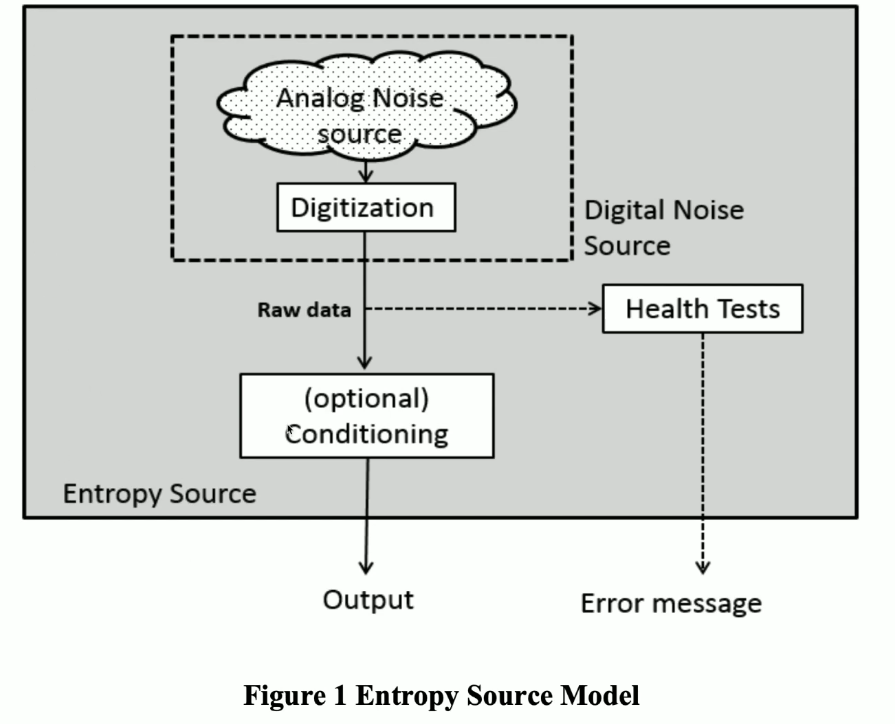
\includegraphics[width=0.8\textwidth]{figures/model_zrodla.png}
    \end{figure}

\end{frame}
%---------------------------------------------------------
\begin{frame}
\frametitle{NIST SP 800-90 B - Conditioning}

    Zalecane metody postprocessingu

    \begin{figure}[H]
      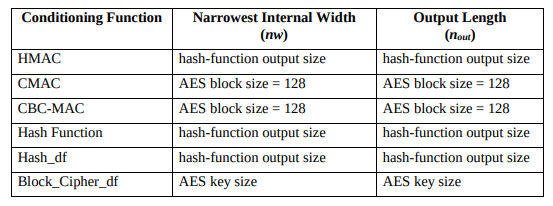
\includegraphics[width=\textwidth]{figures/conditioning.png}
    \end{figure}

\end{frame}
%---------------------------------------------------------
\begin{frame}
\frametitle{NIST SP 800-90 B - Typy testów zdrowia}

\Large
\begin{itemize}
    \item Start-up test - Zapewniają poprawność pracy źródła, przed użyciem w normalnych warunkach.
    \item Continuous tests - detekcja awarii
    \item On-Demand test - np. ponowne wywołanie Start-up test w trakcie pracy
\end{itemize}

\end{frame}
%---------------------------------------------------------
\begin{frame}
\frametitle{NIST SP 800-90 B - Strategia estymacji entropii}

    \begin{figure}[H]
      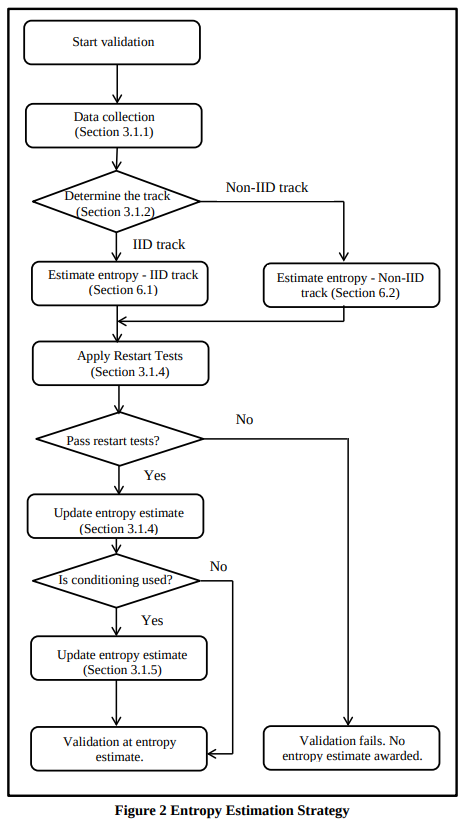
\includegraphics[width=0.35\textwidth]{figures/estymacja.png}
    \end{figure}

\end{frame}
%---------------------------------------------------------
\begin{frame}
\frametitle{NIST SP 800-90 B - Oficjalny program}

    \begin{figure}[H]
      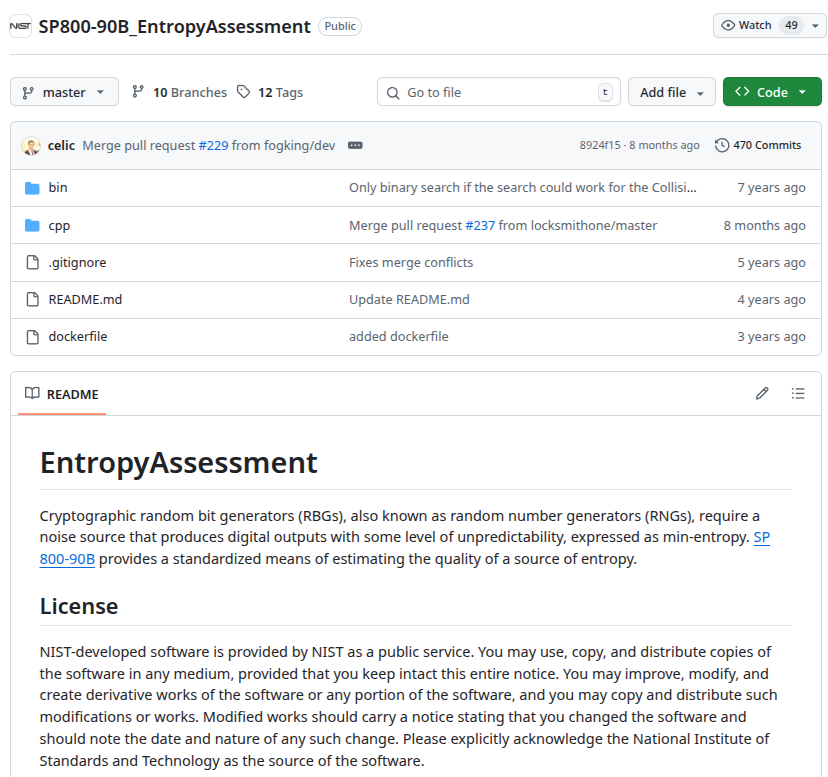
\includegraphics[width=0.8\textwidth]{figures/kod.png}
    \end{figure}

\end{frame}
%---------------------------------------------------------
\begin{frame}
\frametitle{Lista zadań na Luty}

\Large
\begin{enumerate}
    \item Zapoznać się z dokumentacją modułu oscylatora pierścieniowego,
    \item Opracować implementację układu testowego,
    \item Opracować środowisko testowe,
    \item Zebrać pierwsze próbki.
\end{enumerate}
\end{frame}
%---------------------------------------------------------
\section{Przegląd literatury}
%---------------------------------------------------------
\begin{frame}
\frametitle{Normy i standardy}

\begin{enumerate}
    \item NIST SP 800-90B Recommendation for the Entropy Sources Used for Random Bit Generation
\end{enumerate}
\end{frame}
%---------------------------------------------------------
\begin{frame}
\frametitle{Publikacje naukowe}

\begin{enumerate}
    \item Analysis of Ring-Oscillator-based True Random Number Generator on FPGAs Soyeon Choi; Yerin Shin; Hoyoung Yoo
    \item Physical Unclonable Functions (PUF) for IoT Devices Abdulaziz Al-Meer, Saif Al-Kuwari
    \item Hardware-Efficient Configurable RO-Based PUF/TRNG Module for Secure Key Management Santiago Sánchez-Solano ,Luis F. Rojas-Muñoz ,Macarena C. Martínez- and Piedad Brox
\end{enumerate}
\end{frame}
%---------------------------------------------------------
\begin{frame}
\frametitle{Książki}

\begin{enumerate}
    \item Hardware Security: Design, Threats, and Safeguards
    Debdeep Mukhopadhyay, Rajat Subhra Chakraborty
    \item Cryptography Engineering: Design Principles and Practical Applications Niels Ferguson, Bruce Schneier, Tadayoshi Kohno
\end{enumerate}
\end{frame}
%---------------------------------------------------------
\begin{frame}
\frametitle{Dokumentacja techniczna}

\begin{enumerate}
    \item The neoTRNG True Random Number Generator
    \item ENT — Fourmilab Random Sequence Tester
    \item Zynq 7000 SoC Technical Reference Manual
    \item 7 Series FPGAs Configuration User Guide (UG470)
\end{enumerate}
\end{frame}
%---------------------------------------------------------
\begin{frame}
\frametitle{}
\centering{\Huge{\textbf{Dziękuję za uwagę}}}
\end{frame}
%---------------------------------------------------------
\end{document}